\documentclass{article} % simplest latex class that gives nice default structures.  Other classes include standalone, book

% Recommended packages:
\usepackage{listings} % used for listing code

\usepackage{graphicx} % used for importing graphics

\usepackage{amsmath} % Many useful mathematical shortcuts


% Suggested packages:
\usepackage{tikz} % used for drawing figures in LaTeX directly
\usetikzlibrary{automata,calc,arrows} % some useful default tikz packages

\usepackage{enumerate} % used for finer control over enumerate lists

\usepackage{algorithm} % used for specifying algorithms
\usepackage{algpseudocode} % ditto (you need both)

\usepackage{fullpage} % reduces a page's margins to 1cm instead of 1in

\usepackage{mathpazo} % better? fonts

\usepackage{hyperref} % hyperlinks: compile with pdflatex for best results






\begin{document}

\title{Sample \LaTeX\ document}
\author{} % let's keep things anonymous
\date{} % to suppress the date
\maketitle % to actually insert the above three items

\section*{Question 1: Basics} % use section* to suppress numbering

Suggested document structure: give your answers to each question in sections.  Answers to subquestions in subsections, etc. 


\subsection*{Part (a)} % use subsection* to suppress numbering


\LaTeX\ will sort out page layout for you in a sensible/recommended way (e.g.\ page breaks are inserted ``intelligently''), so you shouldn't tinker too much with things, just let \LaTeX\ do its own thing.

\subsection*{Part(b)}
Use \texttt{array} to create aligned math text:

\[
\begin{array}{rlr} %First column aligned right; second column aligned left; third column aligned right
  A &= A \cup A &\quad\mbox{(Idemp.)} \\
  &= (A \cup A) \cup A & \quad\mbox{(Idemp.)}\\
  &= A \cup (A \cup A) & \quad\mbox{(Assoc.)}\\
  &= A \cup A & \quad\mbox{(Idemp.)}
\end{array}
\]

The argument appearing after \verb|\begin{array}| indicates the columns and their alignment.  You can separate them with $\mid$ to obtain vertical column lines.  Use \verb|\hline| to make horizontal ones:

\[
\begin{array}{|c|c|c|c|c|}
\hline
\text{Line} & \text{Assumptions} & \text{Formula} & \text{Justification} & \text{References}\\
\hline
\hline
1 & 1 & (F \land G) & \text{Asmp. I} & 1 \\
\hline
2 & 1 & F & \land\text{ E} & 1\\
\hline
3 & 1 & G & \land\text{ E} & 1\\
\hline
4 & 1 & (G \land F) & \land\text{ I} & 2,3\\
\hline
\end{array}
\]



\section*{Question 2}
The \texttt{listings} package lets you list code verbatim, with some syntax highlighting:
\begin{lstlisting}[language=tex]
\documentclass{article}

\usepackage{listings}

% recursion alert: stack overflow
\end{lstlisting}
A list of supported languages can be found \href{https://en.wikibooks.org/wiki/LaTeX/Source_Code_Listings}{here}.


\section*{Question 3}
The \texttt{enumerate} package lets you do tailored enumerates:
\begin{enumerate}[I]
\item First
\item Second
\item Third
\end{enumerate}

This can be useful if you want to do a simple algorithm:
\begin{enumerate}[Step 1. ]
\item Make a sandwich
\item Eat the sandwich
\end{enumerate}

If you want to break an enumerate with text and then resume, use \verb|\setcounter{enumi}{..}| to start the counter from somewhere specific.  For example
\begin{enumerate}[Step 1. ]
\setcounter{enumi}{-1}
\item Buy sandwich ingredients
\end{enumerate} 


\section*{Question 4: Figures}
You can use \verb|\includegraphics| to import figures from many filetypes: jpg, pdf, eps, png, etc.\texttt{TikZ} is a very useful and powerful package for drawing pictures directly in \LaTeX.  The documentation and library of examples are quite extensive, but the results can be pretty:
\begin{center}
\usetikzlibrary{calc,arrows, shadows}
\begin{tikzpicture}[>=stealth]
\tikzstyle{imgnode}=[rectangle, rounded corners, drop shadow, draw, anchor=north west, minimum width=20pt, minimum height=20pt, fill=white]
\tikzstyle{topnode}=[rectangle, minimum width=20pt, minimum height=10pt]
\tikzstyle{leftchild}= [rectangle, anchor=north west,minimum width=10pt, minimum height=10pt] 
\tikzstyle{rightchild}= [rectangle, anchor=north east,minimum width=10pt, minimum height=10pt]

  \node (A)[topnode] at (0,0) {};
  \node (Ax)[imgnode] at (A.north west){};
  \node (A1)[leftchild] at (A.south west) {};
  \node (A2)[rightchild]  at (A.south east) {};

  \node (B)[topnode] at (2,-1) {};
  \node (Bx)[imgnode] at (B.north west){};
  \node (B1)[leftchild] at (B.south west) {};
  \node (B2)[rightchild]  at (B.south east) {};

  \node (C)[topnode] at (-2,-1) {};
  \node (Cx)[imgnode] at (C.north west){};
  \node (C1)[leftchild] at (C.south west) {};
  \node (C2)[rightchild]  at (C.south east) {};

  \node (D)[topnode] at (-3,-2) {};
  \node (Dx)[imgnode] at (D.north west){};
  \node (D1)[leftchild] at (D.south west) {};
  \node (D2)[rightchild]  at (D.south east) {};

  \node (E)[topnode] at (-1,-2) {};
  \node (Ex)[imgnode] at (E.north west){};
  \node (E1)[leftchild] at (E.south west) {};
  \node (E2)[rightchild]  at (E.south east) {};

  \node (F)[topnode] at (1,-2) {};
  \node (Fx)[imgnode] at (F.north west){};
  \node (F1)[leftchild] at (F.south west) {};
  \node (F2)[rightchild]  at (F.south east) {};

 \draw[*->] let \p1 = (A2), \p2 = (A2.center) in (\x1-2.5,\y2) -- (B);
 \draw[*->] let \p1 = (A1), \p2 = (A1.center) in (\x1+2.5,\y2) -- (C);
 \draw[*->] let \p1 = (C1), \p2 = (C1.center) in (\x1+2.5,\y2) -- (D);
 \draw[*->] let \p1 = (C2), \p2 = (C2.center) in (\x1-2.5,\y2) -- (E);
 \draw[*->] let \p1 = (B1), \p2 = (B1.center) in (\x1+2.5,\y2) -- (F);
 \draw[-] (A1.north west) -- (A2.north east);
 \draw[-] (A1.north east) -- (A1.south east);
 \draw[-] (B1.north west) -- (B2.north east);
 \draw[-] (B1.north east) -- (B1.south east);
 \draw[-] (C1.north west) -- (C2.north east);
 \draw[-] (C1.north east) -- (C1.south east);
 \draw[-] (D1.north west) -- (D2.north east);
 \draw[-] (D1.north east) -- (D1.south east);
 \draw[-] (E1.north west) -- (E2.north east);
 \draw[-] (E1.north east) -- (E1.south east);
 \draw[-] (F1.north west) -- (F2.north east);
 \draw[-] (F1.north east) -- (F1.south east);
\end{tikzpicture}
\end{center}

Here is an example algorithm:  
\begin{algorithmic}
\Procedure{CheckNumbers}{$A$,$B$}
\Statex \Comment{$A$ and $B$ are two lists of integers}
\State count = 0
  \For { $i = 1, \ldots, n$}
     \For {$j=i\ldots m$}
        \If {$A[i]\geq B[j]$}
          \State count = count +1
          \State break
        \EndIf
     \EndFor

\EndFor
\EndProcedure
\end{algorithmic}
It will be inserted exactly where it appears in the document.  This is not recommended because it is better to group the entire algorithm together and ``float'' the group to somewhere where it will all fit: this will make things more readable.  As an example here is a second, much longer, algorithm (see Algorithm~\ref{alg:longer}).
\begin{algorithm}
\begin{algorithmic}
\Procedure{LongerCheckNumbers}{$A$,$B$}
\Statex \Comment{$A$ and $B$ are two lists of integers}
\State count = 0
  \For { $i = 1, \ldots, n$}
     \For {$j=i\ldots m$}
        \If {$A[i]\geq B[j]$}
          \State count = count +1
          \State break
        \EndIf
     \EndFor

\EndFor
\State count = 0
  \For { $i = 1, \ldots, n$}
     \For {$j=i\ldots m$}
        \If {$A[i]\geq B[j]$}
          \State count = count +1
          \State break
        \EndIf
     \EndFor

\EndFor
\State count = 0
  \For { $i = 1, \ldots, n$}
     \For {$j=i\ldots m$}
        \If {$A[i]\geq B[j]$}
          \State count = count +1
          \State break
        \EndIf
     \EndFor

\EndFor
\State count = 0
  \For { $i = 1, \ldots, n$}
     \For {$j=i\ldots m$}
        \If {$A[i]\geq B[j]$}
          \State count = count +1
          \State break
        \EndIf
     \EndFor

\EndFor
\EndProcedure
\end{algorithmic}
\caption{A longer algorithm}\label{alg:longer}
\end{algorithm}

Observe that the \texttt{algorithm} environment also adds nice visual structures around your algorithm.

\subsection*{Part (a)}

You should use \verb|\ref| and \verb|\label| to refer to your algorithm in the text so that the reader can find it.  Note that if you use \verb|\ref| and \verb|\label| you need to compile your latex document twice: the first time grabs all the labels (and puts them into the .aux file) and the second time it can insert the numbers into the file.  Otherwise your references look like this: \ref{unknown}.


You can use \verb|\ref| and \verb|\label| to refer to other parts of your document, including other floating objects (e.g.\ \texttt{figure} for graphics, \texttt{table} for tables). 
\section*{Question 5}
There is almost always a \LaTeX\ package for your typesetting needs.  Most packages are well documented and many of the popular ones have copious amounts of examples of their capabilities.  Google is your friend.

\section*{Question 6: Automata}

With the \texttt{automata} library, drawing automata in tikz is straightforward:
\begin{center}
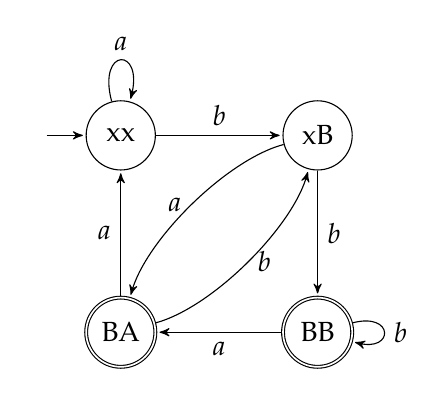
\begin{tikzpicture}[
	>=stealth',  % nice arrowheads
	shorten >=1pt, % don't put arrows all the way to states
	initial text={}, % don't use "Start" to identify the start state
	-> % use arrows
]
\node[initial,state](AA) at (0,0) {xx};
\node[state](AB) at (2.5,0) {xB};
\node[state,accepting](BA) at (0,-2.5){BA};
\node[state,accepting](BB) at (2.5,-2.5){BB};

\path
(AA) edge[loop above] node[above]{$a$} (AA)
(AA) edge node[above]{$b$} (AB)
(AB) edge node[right]{$b$} (BB)
(AB) edge[bend right,looseness=.7] node[left] {$a$} (BA)
(BA) edge[bend right,looseness=.7] node[right] {$b$} (AB)
(BA) edge node[left] {$a$} (AA)
(BB) edge node[below] {$a$} (BA)
(BB) edge[loop right,looseness=6] node[right]{$b$} (BB)
;
\end{tikzpicture}
\end{center}
\end{document}
